\documentclass{article}
\usepackage[utf8]{inputenc}
\usepackage{graphicx}
\usepackage[margin=1.0in]{geometry}

\title{Simulacion Acustica - GEINTRA UAH}
\author{Luis Gonzalez}
\date{Julio 2019}

\begin{document}

\maketitle

\section{Introduction}
Este documento servira como un guia para trabajar con los scripts en MATLAB que ayudan con la simulacion de las salas con varias fuentes y receptores. En resumen, el algoritmo recibe una sala, un array de microfonos, y una lista de ficheros .wav que deseas simular, y genera un .wav simulado por cada combinacion de fuente y microfono cual sea valida en la sala. Se utiliza el Edge Diffraction Toolbox (EDT), un codigo escrito por Peter Svensson de la Norwegian University of Science and Technology, para hacer simulaciones acusticas con reflexiones especulares y difusas. Primero, se haran claro los requisitos que se ocupan para correr el codigo. Despues, se hablara sobre la gestion de archivos despues de la simulacion.

\section{Prerrequisitos}
Para obtener la version mas actual de el codigo, uno puede usar el servicio de version de control que se utiliza el grupo GEINTRA, el CVS. Adentro de cvs, usando el comando:
\begin{center}
    cvs co proyecto-matlab/AcousticRoomSimulation
\end{center}
todos los ficheros seran copiados y archivados localmente. El codigo ha sido escrito y ejecutado en versiones 2018 y 2019 de MATLAB, entonces no es prometido que todas las funciones trabajen como intendidas en versiones anteriores. De todas formas, con la version local, agrega todo el codigo en la carpeta "AplicacionFinal" a el path de tu workspace en MATLAB.
\section{Codigo}
Hay dos scripts que se toman a cargo de las simulaciones. Primero tenemos la fucncion \texttt{calcIR\_simwav}, cual tiene de input: 
\begin{itemize}
    \item \texttt{fpath}: La ruta a el directorio donde se van a guardar los resultados de la simulacion. Esto seran los ficheros de la respuesta de impulso y los setup files de la simulacion, para no confundirse con los ficheros wav que son realmente lo que queremos de al final de la simulacion. 
    \item \texttt{path\_rm}: La ruta a el fichero de la sala. Esto deberia de ser extension .cad, ya que hay problemas con la conversion de .env a .cad que no se pudieron resolver.
    \item \texttt{path\_mc}: La ruta a el fichero de el array de microfonos. La extension sera de tipo .arr.
    \item \texttt{path\_wav}: Una lista de rutas a los ficheros .wav que deseas simular. Si solo quieres simular un fichero, vale con solo usar la ruta como un string.
    \item \texttt{path\_out}: La ruta donde se guardaran los wav simulados.
    \item \texttt{dl}: Se refiere a el "skip" de la cuadricula que se genera en la sala. 
    \item \texttt{start}: El tiempo de incio para el fichero wav. Es decir, dandole un valor de 1 se refiere que el .wav simulado empieza al primer segundo de el .wav original
    \item \texttt{window}: Se refiere a la ventana que quieres grabar. 
\end{itemize}
De todas formas, el codigo tiene un ejemplo de cada input.
Las lineas 130 a 190 se definen variables que pertenecen a las simlaciones, ya como la orden de reflexiones especulares o difusas que deaseas simular. Uno puede cambiar estos parametros manualmente en el codigo dependiendo a como quiere simular la sala.\\\\
Al correr la funcion con los parametros bien definidos, las respuestas del impulso son generadas y guardadas en su destinacion definida. Al final de esta funcion, se llama el segundo script, cual es el que genera los wav simulados. \\\\
El segundo script es \texttt{simwavfromir}. Esta funcion recibe de input una list de todos los ficheros de respuesta al impulso y tambien varios parametros de la funcion principal, como el tiempo de incio y la ventana. Esta es una funcion simple cual genera una convulcion entre la señal de la respuesta al impulso y el wav para generar el audio simulado. Despues, el fichero es guardado en el directorio que hayas definido antes. \\\\
La funcion esta escrita de tal forma en la que si la corres sin parametros, aparece una ventana en la cual podras escojer los ficheros de respuesta al impulso y ficheros wav que quieras simular. Esto espero que sea util si por ejemplo, ya tienes respuestas al impulso y quieres simular mas ficheros wav. 

\section{Gestion de Archivos}
Al correr la funcion de \texttt{calcIR\_simwav} se generan varios ficheros por cada simulacion que sea realizada. El formato en que los ficheros seran guardados es de esta forma:
\begin{center}
    RoomName\_CADName\_src\_x\_y\_z\_mf\_x\_y\_z\_extra
\end{center}
donde extra es un elemento de el set \{1\_1\_edpaths, cadgeo, rdata, sdata, 1\_1\_ir, setup\}. Para nuestro proposito, solo utilizamos los resultados de el fichero de ir, la respuesta al impulso, pero el resto de los ficheros son necesarios para correr la simulacion.\\\\
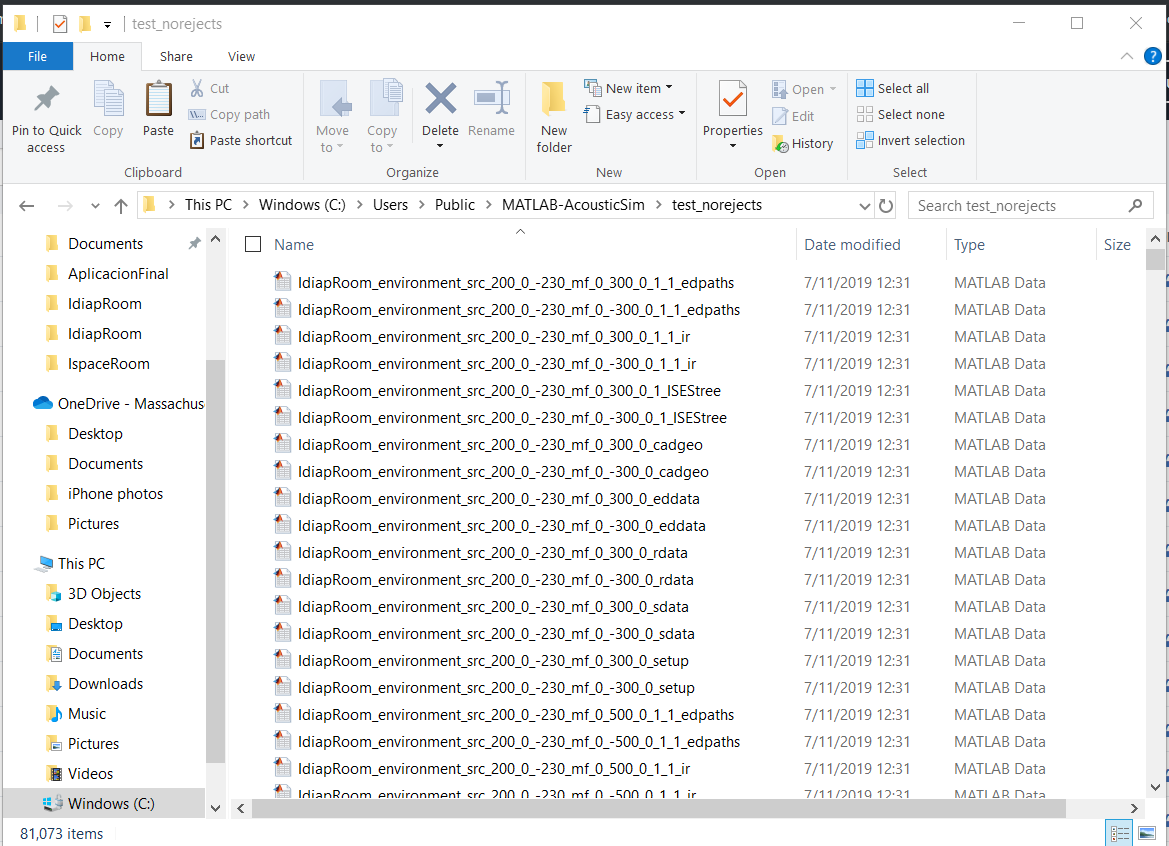
\includegraphics[width=0.9\textwidth]{filemanage.png}

\section{Simulacion}
Hay dos formas de utilizar las funciones que fueron escritas. El primer enfoque se trata de escribir un script que llame a calcIR\_simwav multiples veces con la lista de todos los wav que quieras simular. De esta forma, solo tienes que llamar a la funcion una vez y tendras los resultados. Lo que tendra uno que hacer es generar la lista de rutas a los ficheros wav.\\\\
Otra forma de generar los wav simulados seria llamar la funcion con solo la sala, el array de microfonos, y el $\Delta l$ de la cuadricula. De esta forma tendras las respuestas al impulso y podras llamar la otra funcion y selecionar las respuestas al impulso junto con los wav que quieras simular. 

\section{Addendum}
Al generar los puntos de la sala, se generan cordenadas de una caja, y despues se usa una funcion que verifica si el punto esta dentro de la sala. Si es el caso que el punto esta fuera de la sala, se generera un warning en la ventana de comando. Igualmente cuando una simulacion no se pueda realizar dudo a que la fuente/microfono esten muy cercanos, se genera un warning y se trata de simular el punto siguiente. Si la simulacion llega a un error inesperado, el codigo para y tendra que correrse de nuevo. Esto se hace para no generar simulaciones erroneas.  



\end{document}
